% !TeX spellcheck = es_ES
% !TeX encoding = UTF-8
\documentclass[10pt, a4paper, landscape]{article}

% ----- packages -----
\usepackage{amsmath} % AMS mathematical facilities for LaTeX
\usepackage{enumitem} % Control layout of itemize, enumerate, description
\usepackage{fancyhdr} % Extensive control of page headers and footers in LaTeX2
\usepackage{geometry} % Flexible and complete interface to document dimensions
\usepackage{graphicx} % Enhanced support for graphics
\usepackage{hyperref} % Extensive support for hypertext in LaTeX
\usepackage{multicol} % Intermix single and multiple columns
\usepackage{parskip} % Layout with zero \parindent, non-zero \parskip
\usepackage{tikz} % Create PostScript and PDF graphics in TeX
\usepackage{titlesec} % Select alternative section titles

% ----- pdf metadata -----
\hypersetup{
	pdftitle={Hoja de Referencia Series Temporales},
	pdfsubject={The Econometrics Cheat Sheet Project - marcelomijas - CC-BY-4.0},
	pdfauthor={Marcelo Moreno Porras},
	pdfkeywords={statistics, latex, economics, cheatsheet, econometrcis, ols-regression, economic-modelling},
	pdfduplex={DuplexFlipShortEdge}
}

% ----- random seed -----
\pgfmathsetseed{12}

% ----- custom commands -----
\DeclareMathOperator{\E}{E}
\DeclareMathOperator{\Var}{Var}
\DeclareMathOperator{\se}{ee}
\DeclareMathOperator{\Cov}{Cov}
\DeclareMathOperator{\Corr}{Corr}

% ----- page customization -----
\geometry{margin=1cm} % margins config
\pagenumbering{gobble} % remove page numeration
\setlength{\parskip}{0cm} % paragraph spacing
% title spacing
\titlespacing{\section}{0pt}{2ex}{1ex}
\titlespacing{\subsection}{0pt}{1ex}{0ex}
\titlespacing{\subsubsection}{0pt}{0.5ex}{0ex}

% ----- footer -----
\pagestyle{fancy}
\renewcommand{\headrulewidth}{0pt}
\cfoot{\href{https://github.com/marcelomijas/econometrics-cheatsheet}{\normalfont \footnotesize TS-25.08.2-ES - github.com/marcelomijas/econometrics-cheatsheet - CC-BY-4.0 license}}
\setlength{\footskip}{12pt}

% ----- document -----
\begin{document}

\begin{multicols}{3}

\begin{center}
	\textbf{\LARGE \href{https://github.com/marcelomijas/econometrics-cheatsheet}{Hoja de Referencia Series Temporales}}

	{\footnotesize Por Marcelo Moreno Porras - Universidad Rey Juan Carlos}

	{\footnotesize The Econometrics Cheat Sheet Project}
\end{center}

\section*{Conceptos básicos}

\subsection*{Definiciones}

\textbf{Serie temporal} - sucesión de observaciones ordenadas en el tiempo con una frecuencia fija.

Dado el formato de una serie temporal:

\begin{itemize}[leftmargin=*]
	\item \textbf{Punto en el tiempo (stock)} - se registra un único valor para cada período.
	\item \textbf{Agregado (flujo)} - los valores representan totales o promedios a lo largo del período.
	\item \textbf{Rango/intervalo (OHLC)} - cada período registra múltiples estadísticas, como \textit{min, max, open, close}.
\end{itemize}

\textbf{Proceso estocástico} - es una secuencia de variables aleatorias que están indexadas en el tiempo.

\subsection*{Componentes de una serie temporal}

\begin{itemize}[leftmargin=*]
	\item \textbf{Tendencia} - movimiento general a l/p de una serie.
	\item \textbf{Variaciones estacionales} - oscilaciones periódicas producidas en un período igual o inferior al año, y pueden ser fácilmente identificadas en diferentes años (usualmente resultado de la climatología).
	\item \textbf{Ciclo} - oscilaciones periódicas producidas en un periodo mayor al año (son resultado del ciclo económico).
	\item \textbf{Variaciones residuales} - movimientos que no siguen una oscilación periódica identificable (eventos irreg.)
\end{itemize}

\subsection*{Tipos de modelos de series temporales}

\begin{itemize}[leftmargin=*]
	\item \textbf{Modelos estáticos} - la relación entre \( y \) y \( x \) es contemporánea. Conceptualmente:
	\begin{center}
		\( y_{t} = \beta_{0} + \beta_{1} x_{t} + u_{t} \)
	\end{center}
	\item \textbf{Modelos de rezagos distribuidos} - la relación entre \( y \) y \( x \) no es contemporánea. Conceptualmente:
	\begin{center}
		\( y_{t} = \beta_{0} + \beta_{1} x_{t} + \beta_{2} x_{t - 1} + \cdots + \beta_{s} x_{t - (s - 1)} + u_{t} \)
	\end{center}
	El efecto acumulado a largo plazo en \( y \) cuando \( \Delta x \) es:
	\begin{center}
		\( \beta_{1} + \beta_{2} + \cdots + \beta_{s} \)
	\end{center}
	\item \textbf{Modelos dinámicos} - rezagos de la variable dependiente (endogeneidad). Conceptualmente:
	\begin{center}
		\( y_{t} = \beta_{0} + \beta_{1} y_{t - 1} + \cdots + \beta_{s} y_{t - s} + u_{t} \)
	\end{center}
	\item Combinación de lo anterior, como modelos de rezagos distribuidos racionales (rezagos distribuidos + dinámicos).
\end{itemize}

\columnbreak

\section*{Supuestos y propiedades}

\subsection*{Supuestos MCO bajo series temporales}

Bajo estos supuestos, los estimadores de los parámetros MCO presentarán buenas propiedades. \textbf{Supuestos Gauss-Markov} extendidos para series temporales:

\begin{enumerate}[leftmargin=*, label=t\arabic{*}.]
	\item \textbf{Linealidad de parámetros y dependencia débil}.
	\begin{enumerate}[leftmargin=*, label=\alph{*}.]
		\item \( y_{t} \) debe ser una función lineal de \( \beta \).
		\item El proceso estocástico \( \lbrace (x_{t}, y_{t}) : t = 1, 2, \ldots, T \rbrace \) es estacionario y débilmente dependiente.
	\end{enumerate}
	\item \textbf{No colinealidad perfecta}.
	\begin{itemize}[leftmargin=*]
		\item No hay variables independientes que sean constantes: \( \Var(x_{j}) \neq 0, \; \forall j = 1, \ldots, k \)
		\item No hay una relación lineal exacta entre variables independientes.
	\end{itemize}
	\item \textbf{Media condicional cero y correlación cero}.
	\begin{enumerate}[leftmargin=*, label=\alph{*}.]
		\item No hay errores sistemáticos: \( \E(u \mid x_{1}, \ldots, x_{k}) = \E(u) = 0 \rightarrow \) \textbf{exogeneidad fuerte} (a implica b).
		\item No hay variables relevantes no incluidas en el modelo: \( \Cov(x_{j} , u) = 0, \; \forall j = 1, \ldots, k \rightarrow \) \textbf{exogeneidad débil}.
	\end{enumerate}
	\item \textbf{Homocedasticidad}. La variabilidad de los resid. es igual para cualquier nivel de \( x \): \( \Var(u \mid x_{1}, \ldots, x_{k}) = \sigma_{u}^{2} \)
	\item \textbf{No autocorrelación}. Los residuos no contienen información sobre otros residuos: \\
	\( \Corr(u_{t}, u_{s} \mid x_{1}, \ldots, x_{k}) = 0, \; \forall t \neq s \)
	\item \textbf{Normalidad}. Los residuos son independientes e idénticamente distribuidos (\textbf{i.i.d.}): \( u \sim \mathcal{N} (0, \sigma_{u}^{2}) \)
	\item \textbf{Tamaño de datos}. El número de observaciones disponibles debe ser mayor a \( (k + 1) \) parámetros a estimar. (Ya satisfecho bajo situaciones asintóticas)
\end{enumerate}

\subsection*{Propiedades asintóticas de MCO}

Bajo los supuestos del modelo econométrico y el Teorema Central del Límite:

\begin{itemize}[leftmargin=*]
	\item De t1 a t3a: MCO es \textbf{insesgado}. \( \E(\hat{\beta}_{j}) = \beta_{j} \)
	\item De t1 a t3: MCO es \textbf{consistente}. \( \operatorname{plim}(\hat{\beta}_{j}) = \beta_{j} \) (a t3b sin t3a, exogeneidad débil, insesg. y consistente).
	\item De t1 a t5: \textbf{normalidad asintótica} de MCO (entonces, t6 es necesariamente satisfecho): \( u \underset{a}{\sim} \mathcal{N} (0, \sigma_{u}^{2}) \)
	\item De t1 a t5: \textbf{estimador insesgado} de \( \sigma_{u}^{2} \). \( \E(\hat{\sigma}_{u}^{2}) = \sigma^{2}_{u} \)
	\item De t1 a t5: MCO es MELI (Mejor Estimador Lineal Insesgado, \textcolor{blue}{BLUE} en inglés) or \textbf{eficiente}.
	\item De t1 a t6: contrastes de hipótesis e intervalos de confianza son fiables.
\end{itemize}

\columnbreak

\section*{Tendencia y estacionalidad}

\textbf{Regresión espuria} - es cuando la relación entre \( y \) y \( x \) es debida a factores que afectan a \( y \) y que tienen correlación con \( x \), \( \Corr(x_{j}, u) \neq 0 \). Es el \textbf{incumplimiento de t3}.

\subsection*{Tendencia}

Dos series temporales pueden tener la misma (o contraria) tendencia, lo que lleva a altos niveles de correlación. Esto provoca una falsa apariencia de causalidad; el problema es \textbf{regresión espuria}. Dado el modelo:

\begin{center}
	\( y_{t} = \beta_{0} + \beta_{1} x_{t} + u_{t} \)
\end{center}

donde:

\begin{center}
	\( y_{t} = \alpha_{0} + \alpha_{1} \text{Tendencia} + v_{t} \)

	\( x_{t} = \gamma_{0} + \gamma_{1} \text{Tendencia} + v_{t} \)
\end{center}

Añadir una tendencia al modelo puede resolver el problema:

\begin{center}
	\( y_{t} = \beta_{0} + \beta_{1} x_{t} + \beta_{2} \text{Tendencia} + u_{t} \)
\end{center}

Una tendencia puede ser lineal o no lineal (cuadrática, cúbica, exponencial, etc.)

Otra manera, es hacer uso del \textbf{filtro Hodrick-Prescott} y extraer la tendencia y el componente cíclico.

\subsection*{Estacionalidad}

\setlength{\multicolsep}{0pt}
\begin{multicols}{2}

Una serie temporal puede manifestar estacionalidad. Esto es, que la serie está sujeta a variaciones estacionales o patrones usualmente relacionados al clima.

\columnbreak

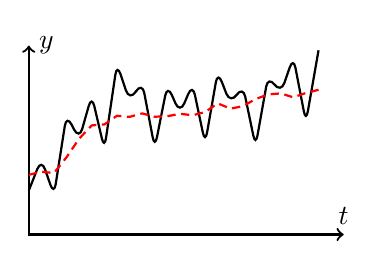
\begin{tikzpicture}[scale=0.20]
	\draw [thick, <->] (0, 12) node [anchor=west] {\( y \)} -- (0, 0) -- (20, 0) node [anchor=south] {\( t \)};
	\draw [thick, black, rounded corners] 
	(0.0, 2.79) -- (0.8, 4.81) -- 
	(1.6, 2.50) -- (2.4, 7.61) -- 
	(3.2, 6.03) -- (4.0, 8.84) -- 
	(4.8, 5.42) -- (5.6, 10.85) -- 
	(6.4, 8.47) -- (7.2, 9.69) -- 
	(8.0, 5.48) -- (8.8, 9.51) -- 
	(9.6, 7.68) -- (10.4, 9.57) -- 
	(11.2, 5.78) -- (12.0, 10.36) -- 
	(12.8, 8.29) -- (13.6, 9.45) -- 
	(14.4, 5.60) -- (15.2, 10.09) -- 
	(16.0, 8.96) -- (16.8, 11.28) -- 
	(17.6, 7.13) -- (18.4, 11.70);
	\draw [thick, red, densely dashed, line join=round] 
	(0.0, 3.79) -- (0.8, 3.99) -- 
	(1.6, 3.90) -- (2.4, 4.91) -- 
	(3.2, 6.09) -- (4.0, 6.93) -- 
	(4.8, 6.99) -- (5.6, 7.54) -- 
	(6.4, 7.47) -- (7.2, 7.69) -- 
	(8.0, 7.48) -- (8.8, 7.51) -- 
	(9.6, 7.67) -- (10.4, 7.57) -- 
	(11.2, 7.78) -- (12.0, 8.33) -- 
	(12.8, 7.99) -- (13.6, 8.15) -- 
	(14.4, 8.60) -- (15.2, 8.90) -- 
	(16.0, 8.96) -- (16.8, 8.71) -- 
	(17.6, 8.99) -- (18.4, 9.19);
\end{tikzpicture}

\end{multicols}

Por ejemplo, el PIB (negro) es usualmente mayor en verano y menor en invierno. Serie ajustada estacionalmente ({\color{red} rojo discontinuo}) en comparación.

\begin{itemize}[leftmargin=*]
	\item La regresión de series de tiempo que presentan estacionalidad puede conducir a \textbf{resultados espurios}.
\end{itemize}

Un \textbf{ajuste estacional} sencillo es crear variables estacionales binarias y añadirlas al modelo. Por ejemplo, una serie trimestral (\( Q q_{t} \) son variables binarias):

\begin{center}
	\( y_{t} = \beta_{0} + \beta_{1} Q2_{t} + \beta_{2} Q3_{t} + \beta_{3} Q4_{t} + \beta_{4} x_{1t} + \cdots + \beta_{k} x_{kt} + u_{t} \)
\end{center}

Otro método es ajustar estacionalmente (sa) las variables, y entonces, hacer la regresión con las variables ajustadas:

\begin{center}
	\( z_{t} = \beta_{0} + \beta_{1} Q2_{t} + \beta_{2} Q3_{t} + \beta_{3} Q4_{t} + v_{t} \rightarrow \hat{v}_{t} + \E(z_{t}) = \hat{z}_{t}^{sa} \)

	\( \hat{y}_{t}^{sa} = \beta_{0} + \beta_{1} \hat{x}_{1t}^{sa} + \cdots + \beta_{k} \hat{x}_{kt}^{sa} + u_{t} \)
\end{center}

Hay métodos mucho mejores y complejos para ajustar estacionalmente, como el \textbf{X-13ARIMA-SEATS}.

\columnbreak

\section*{Autocorrelación}

El residuo de cualquier observación, \( u_{t} \), está correlacionado con el residuo de cualquier otra observación. Las observaciones no son independientes. \textbf{Incumplimiento} de \textbf{t5}.

\begin{center}
	\( \Corr(u_{t}, u_{s} \mid x_{1}, \ldots, x_{k}) = \Corr(u_{t}, u_{s}) \neq 0, \; \forall t \neq s \)
\end{center}

\subsection*{Consecuencias}

\begin{itemize}[leftmargin=*]
	\item Estimadores MCO son insesgados.
	\item Estimadores MCO son consistentes.
	\item MCO ya \textbf{no es eficiente}, pero sigue siendo ELI (Estimador Lineal Insesgado).
	\item La \textbf{estimación de la varianza} de los estimadores es \textbf{sesgada}: la construcción de intervalos de confianza y contraste de hipótesis no son fiables.
\end{itemize}

\subsection*{Detección}

\textbf{Gráficos de dispersión} - patrones en \( u_{t - 1} \) vs. \( u_{t} \).

\setlength{\multicolsep}{0pt}
\setlength{\columnsep}{6pt}
\begin{multicols}{3}

\begin{center}
	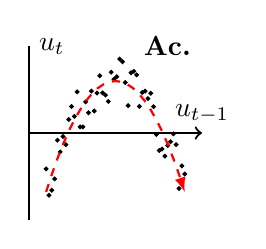
\begin{tikzpicture}[scale=0.11]
		\node at (16, 20) {\textbf{Ac.}}; 
		\draw [thick, ->] (0, 10) -- (20, 10) node [anchor=south] {\( u_{t - 1} \)}; 
		\draw [thick, -] (0, 0) -- (0, 20) node [anchor=west] {\( u_{t} \)}; 
		\draw plot [only marks, mark=*, mark size=6, domain=2:18, samples=50] (\x, {-0.2*(\x - 10)^2 + 13 + 6*rnd}); 
		\draw [thick, dashed, red, -latex] plot [domain=2:18] (\x, {-0.2*(\x - 10)^2 + 16});
	\end{tikzpicture}
\end{center}

\columnbreak

\begin{center}
	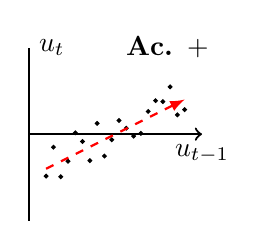
\begin{tikzpicture}[scale=0.11]
		\node at (16, 20) {\textbf{Ac. \( + \)}}; 
		\draw [thick, ->] (0, 10) -- (20, 10) node [anchor=north] {\( u_{t - 1} \)}; 
		\draw [thick, -] (0, 0) -- (0, 20) node [anchor=west] {\( u_{t} \)}; 
		\draw plot [only marks, mark=*, mark size=6, domain=2:18, samples=20] (\x, {5*rnd + 2.5 + 0.5*\x}); 
		\draw [thick, dashed, red, -latex] plot [domain=2:18] (\x, {5 + 0.5*\x});
	\end{tikzpicture}
\end{center}

\columnbreak

\begin{center}
	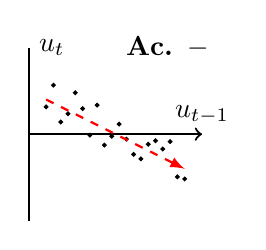
\begin{tikzpicture}[scale=0.11]
		\node at (16, 20) {\textbf{Ac. \( - \)}}; 
		\draw [thick, ->] (0, 10) -- (20, 10) node [anchor=south] {\( u_{t - 1} \)}; 
		\draw [thick, -] (0, 0) -- (0, 20) node [anchor=west] {\( u_{t} \)}; 
		\draw plot [only marks, mark=*, mark size=6, domain=2:18, samples=20] (\x, {5*rnd + 12.5 - 0.5*\x}); 
		\draw [thick, dashed, red, -latex] plot [domain=2:18] (\x, {15 - 0.5*\x});
	\end{tikzpicture}
\end{center}

\end{multicols}

\begin{multicols}{2}

\textbf{Correlograma} - función de autocorrelación (FAC) y el FAC parcial (FACP).

\columnbreak

\begin{itemize}[leftmargin=*]
	\item Eje Y: correlación.
	\item Eje X: núm. de retardo.
	\item Área gris: \( \pm 1.96 / T^{0.5} \)
\end{itemize}

\end{multicols}

\begin{center}
	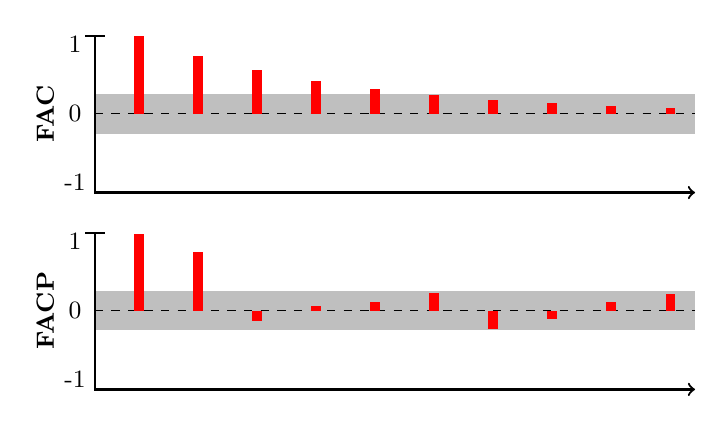
\begin{tikzpicture}[scale=0.25]
		% acf plot
		\node at (-2.5, 14) {\small \rotatebox{90}{\textbf{FAC}}}; 
		\node at (-1, 17.5) {\small 1};
		\node at (-1, 14) {\small 0};
		\node at (-1, 10.5) {\small -1}; 
		\fill [lightgray] (0, 13) rectangle (30.5, 15); 
		\draw [dashed, thin] (0, 14) -- (30.5, 14); 
		\draw [thick, |->] (0, 18) -- (0, 10) -- (30.5, 10);
		\fill [red] (2, 14) rectangle (2.5, 17.95);
		\fill [red] (5, 14) rectangle (5.5, 16.96);
		\fill [red] (8, 14) rectangle (8.5, 16.22); 
		\fill [red] (11, 14) rectangle (11.5, 15.67);
		\fill [red] (14, 14) rectangle (14.5, 15.25);
		\fill [red] (17, 14) rectangle (17.5, 14.94);
		\fill [red] (20, 14) rectangle (20.5, 14.70);
		\fill [red] (23, 14) rectangle (23.5, 14.53);
		\fill [red] (26, 14) rectangle (26.5, 14.40);
		\fill [red] (29, 14) rectangle (29.5, 14.30);
		% pacf plot
		\node at (-2.5, 4) {\small \rotatebox{90}{\textbf{FACP}}};
		\node at (-1, 7.5) {\small 1};
		\node at (-1, 4) {\small 0};
		\node at (-1, 0.5) {\small -1};
		\fill [lightgray] (0, 3) rectangle (30.5, 5);
		\draw [dashed, thin] (0, 4) -- (30.5, 4);
		\draw [thick, |->] (0, 8) -- (0, 0) -- (30.5, 0);
		\fill [red] (2, 4) rectangle (2.5, 7.90);
		\fill [red] (5, 4) rectangle (5.5, 7.00);
		\fill [red] (8, 4) rectangle (8.5, 3.47);
		\fill [red]	(11, 4) rectangle (11.5, 4.24);
		\fill [red] (14, 4) rectangle (14.5, 4.43);
		\fill [red] (17, 4) rectangle (17.5, 4.89);
		\fill [red] (20, 4) rectangle (20.5, 3.09);
		\fill [red] (23, 4) rectangle (23.5, 3.58);
		\fill [red] (26, 4) rectangle (26.5, 4.46);
		\fill [red] (29, 4) rectangle (29.5, 4.86);
	\end{tikzpicture}
\end{center}

\begin{itemize}[leftmargin=*]
	\item \textbf{Proceso \( \text{MA}(q) \)}. \underline{FAC}: sólo los \( q \) primeros coeficientes son significativos, el resto se anulan bruscamente. \underline{FACP}: decrecimiento rápido exponencial atenuado u ondas sinusoidales.
	\item \textbf{Proceso \( \text{AR}(p) \)}. \underline{FAC}: decrecimiento rápido exponencial atenuado u ondas sinusoidales. \underline{FACP}: sólo los \( p \) primeros coeficientes son significativos, el resto se anulan bruscamente.
\end{itemize}

\columnbreak

\begin{itemize}[leftmargin=*]
	\item \textbf{Proceso \( \text{ARMA}(p, q) \)}. \underline{FAC} y \underline{FACP}: los coeficientes no se anulan bruscamente y presentan un decrecimiento rápido.
\end{itemize}

Si los coeficientes de la FAC no decaen rápidamente, hay claro indicio de falta de estacionariedad en media.

\textbf{Contrastes} - Generalmente, \( H_{0} \): No autocorrelación.

Suponiendo que \( u_{t} \) sigue un proceso AR(1):

\begin{center}
	\( u_{t} = \rho_{1} u_{t - 1} + \varepsilon_{t} \)
\end{center}

donde \( \varepsilon_{t} \) es ruido blanco.

\begin{itemize}[leftmargin=*]
	\item \textbf{Prueba t AR(1)} (regresores exógenos):
	\begin{center}
		\( t = \dfrac{\hat{\rho}_{1}}{\se(\hat{\rho}_{1})} \sim t_{T - k - 1, \alpha / 2} \)
	\end{center}
	\( H_{1} \): Autocorrelación de orden uno, AR(1).
\end{itemize}

\begin{itemize}[leftmargin=*]
	\item \textbf{Estadístico Durbin-Watson} (regresores exógenos y normalidad de residuos):
	\begin{center}
		\( d = \dfrac{\sum_{t = 2}^{n} (\hat{u}_{t} - \hat{u}_{t - 1})^{2}}{\sum_{t = 1}^{n} \hat{u}_{t}^{2}} \approx 2 \cdot (1 - \hat{\rho}_{1}) \)
	\end{center}
	Donde \( 0 \leq d \leq 4 \)

	\( H_{1} \): Autocorrelación de orden uno, AR(1).
\end{itemize}

\begin{center}
	\begin{tabular}{ c | c | c | c }
		\( d = \)          & 0 & 2 & 4  \\ \hline
		\( \rho \approx \) & 1 & 0 & -1
	\end{tabular}

	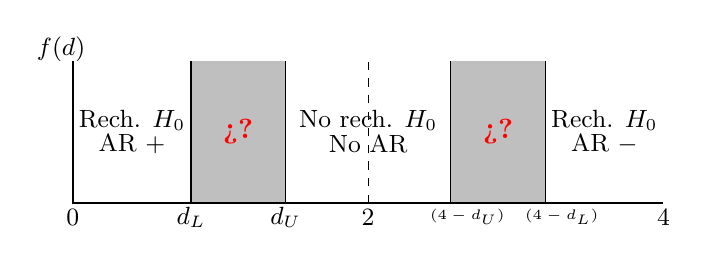
\begin{tikzpicture}[scale=0.3]
		\fill [lightgray] (5, 0) rectangle (9, 6); 
		\draw (5, 0) -- (5, 6);
		\draw (9, 0) -- (9, 6);
		\fill [lightgray] (16, 0) rectangle (20, 6);
		\draw (16, 0) -- (16, 6);
		\draw (20, 0) -- (20, 6);
		\draw [thick] (0, 6) -- (0, 0) -- (25, 0);
		\draw [dashed] (12.5, 0) -- (12.5, 6);
		\node at (-0.5, 6.5) {\small \( f(d) \)};
		\node at (0, -0.6) {\small 0};
		\node at (5, -0.6) {\small \( d_{L} \)};
		\node at (9, -0.6) {\small \( d_{U} \)};
		\node at (12.5, -0.6) {\small 2};
		\node at (16.7, -0.6) {\tiny \( (4 - d_{U}) \)};
		\node at (20.7, -0.6) {\tiny \( (4 - d_{L}) \)};
		\node at (25, -0.6) {\small 4};
		\node at (2.5, 3.5) {\small Rech. \( H_{0} \)};
		\node at (2.5, 2.5) {\small AR \( + \)};
		\node [text=red] at (7, 3) {\textbf{¿?}};
		\node at (12.5, 3.5) {\small No rech. \( H_{0} \)};
		\node at (12.5, 2.5) {\small No AR};
		\node [text=red] at (18, 3) {\textbf{¿?}};
		\node at (22.5, 3.5) {\small Rech. \( H_{0} \)};
		\node at (22.5, 2.5) {\small AR \( - \)};
	\end{tikzpicture}
\end{center}

\begin{itemize}[leftmargin=*]
	\item \textbf{h de Durbin} (regresores endógenos):
	\begin{center}
		\( h = \hat{\rho} \cdot \sqrt{\dfrac{T}{1 - T \cdot \upsilon}} \)
	\end{center}
	donde \( \upsilon \) es la varianza estimada del coeficiente asociado a la variable endógena.

	\( H_{1} \): Autocorrelación de orden uno, AR(1).
\end{itemize}

\begin{itemize}[leftmargin=*]
	\item \textbf{Prueba Breusch-Godfrey} (regresores endógenos): puede detectar procesos \( \text{MA}(q) \) y \( \text{AR}(p) \) (\( \varepsilon_{t} \) ruido b.):
	\begin{itemize}[leftmargin=*]
		\item \( \text{MA}(q) \): \( u_{t} = \varepsilon_{t} - m_{1} u_{t - 1} - \cdots - m_{q} u_{t - q} \)
		\item \( \text{AR}(p) \): \( u_{t} = \rho_{1} u_{t - 1} + \cdots + \rho_{p} u_{t - p}+ \varepsilon_{t} \)
	\end{itemize}
	Bajo \( H_{0} \): No autocorrelación:
	\begin{center}
		\( \hfill T \cdot R_{\hat{u}_t}^{2} \underset{a}{\sim} \chi_{q}^{2} \hfill \text{or} \hfill T \cdot R_{\hat{u}_t}^{2} \underset{a}{\sim} \chi_{p}^{2} \hfill \)
	\end{center}
	\( H_{1} \): Autocorrelación de orden \( q \) (ó \( p \)).
\end{itemize}

\begin{itemize}[leftmargin=*]
	\item \textbf{Prueba Ljung-Box Q}:

	\( H_{1} \): Autocorrelación hasta orden \( h \).
\end{itemize}

\columnbreak

\subsection*{Corrección}

\begin{itemize}[leftmargin=*]
	\item Usar MCO con un estimador de la matriz de varianzas-covarianzas \textbf{robusto a la heterocedasticidad y autocorrelación} (HAC), por ejemplo, la propuesta de \textbf{Newey-West}.
	\item Usar \textbf{Mínimos Cuadrados Generalizados} (MCG). Suponiendo \( y_{t} = \beta_{0} + \beta_{1} x_{t} + u_{t} \), con \( u_{t} = \rho u_{t - 1} + \varepsilon_{t} \), donde \( \lvert \rho \rvert < 1 \) y \( \varepsilon_{t} \) es \underline{ruido blanco}.
	\begin{itemize}[leftmargin=*]
		\item Si \( \rho \) es \textbf{conocido}, usar \textbf{modelo cuasi-diferenciado}:
		\begin{center}
			\( y_{t} - \rho y_{t - 1}= \beta_{0} (1 - \rho) + \beta_{1} (x_{t} - \rho x_{t - 1}) + u_{t} - \rho u_{t - 1} \)

			\( y_{t}^{*} = \beta_{0}^{*} + \beta_{1}' x_{t}^{*} + \varepsilon_{t} \)
		\end{center}
		donde \( \beta_{1}' = \beta_{1} \); y estimarlo por MCO.
		\item Si \( \rho \) es \textbf{desconocido}, estimarlo -por ejemplo- el \textbf{método iterativo de Cochrane-Orcutt} (el método de Prais-Winsten también es bueno):
		\begin{enumerate}[leftmargin=*]
			\item Obtener \( \hat{u}_{t} \) del modelo original.
			\item Estimar \( \hat{u}_{t} = \rho \hat{u}_{t - 1} + \varepsilon_{t} \) y obtener \( \hat{\rho} \).
			\item Crear un modelo cuasi-diferenciado:
			\begin{center}
				\( y_{t} - \hat{\rho}y_{t - 1} = \beta_{0} (1 - \hat{\rho}) + \beta_{1} (x_{t} - \hat{\rho} x_{t - 1}) + u_{t} - \hat{\rho}u_{t - 1} \)

				\( y_{t}^{*} = \beta_{0}^{*} + \beta_{1}' x_{t}^{*} + \varepsilon_{t} \)
			\end{center}
			donde \( \beta_{1}' = \beta_{1} \); y estimarlo por MCO.
			\item Obtener \( \hat{u}_{t}^{*} = y_{t} - (\hat{\beta}_{0}^{*} + \hat{\beta}_{1}' x_{t}) \neq y_{t} - (\hat{\beta}_{0}^{*} + \hat{\beta}_{1}' x_{t}^{*}) \).
			\item Repetir desde el paso 2. El algoritmo termina cuando los parámetros estimados varían muy poco entre iteraciones.
		\end{enumerate}
	\end{itemize}
	\item Si no se arregla, buscar \textbf{fuerte dependencia} en la serie.
\end{itemize}

\section*{Suavizado exponencial}

Dado \( \{ y_{t} \} \), la serie suavizada \( \{ f_{t} \} \):

\begin{center}
	\( f_{t} = \alpha y_{t} + (1 - \alpha) f_{t - 1} \)
\end{center}

donde \( 0 < \alpha < 1 \) es el factor de suavizado y \( f_{0} = y_{0} \).

\section*{Predicciones}

Dos tipos de predicciones:

\begin{itemize}[leftmargin=*]
	\item Valor medio de \( y \) para un valor específico de \( x \).
	\item Valor individual de \( y \) para un valor específico de \( x \).
\end{itemize}

\textbf{U de Theil} - compara los resultados pronosticados con los de la previsión con datos históricos mínimos.

\begin{center}
	\( U = \sqrt{\frac{\sum_{t = 1}^{T - 1} \left( \frac{\hat{y}_{t + 1} - y_{t + 1}}{y_{t}} \right)^{2}}{\sum_{t = 1}^{T - 1} \left( \frac{y_{t + 1} - y_{t}}{y_{t}} \right)^{2}}} \)
\end{center}

\begin{itemize}[leftmargin=*]
	\item \( < 1 \): La predicción es mejor que adivinar.
	\item \( = 1 \): La predicción es tan buena como adivinar.
	\item \( > 1 \): La predicción es peor que adivinar.
\end{itemize}

\columnbreak

\section*{Estacionariedad}

La estacionariedad permite reconocer relaciones --inalteradas en el tiempo-- entre variables.

\begin{itemize}[leftmargin=*]
	\item \textbf{Proceso estacionario} (estacionariedad estricta) - la distribución de probabilidad conjunta del proceso permanece inalterada al desplazarse \( h \) periodos.
	\item \textbf{Proceso no estacionario} - por ejemplo, una serie con tendencia, donde al menos la media cambia con el tiempo.
	\item \textbf{Proceso estacionario en covarianza} - es una forma más débil de estacionariedad:
	\begin{itemize}[leftmargin=*]
		\begin{multicols}{2}
			\item \( \E(x_{t}) \) es constante.
		\columnbreak
			\item \( \Var(x_{t}) \) es constante.
		\end{multicols}
		\item Para cualquier \( t, h \geq 1 \), \( \Cov(x_{t}, x_{t + h}) \) depende sólo de \( h \), no de \( t \).
	\end{itemize}
\end{itemize}

\section*{Dependencia débil}

La dependencia débil reemplaza el supuesto de muestreo aleatorio en series temporales.

\begin{itemize}[leftmargin=*]
	\item Un proceso estacionario \( \{ x_{t} \} \) es \textbf{débilmente dependiente} cuando \( x_{t} \) y \( x_{t + h} \) son casi independientes a medida que \( h \) aumenta sin límite.
	\item Un proceso estacionario en covarianza es \textbf{débilmente dependiente} si la correlación entre \( x_{t} \) y \( x_{t + h} \) tiende a 0 lo suficientemente rápido cuando \( h \rightarrow \infty \) (no están asintóticamente correlacionados).
\end{itemize}

Los procesos débilmente dependientes se llaman \textbf{integrados de orden cero}, I(0). Algunos ejemplos:

\begin{itemize}[leftmargin=*]
	\item \textbf{Media móvil} - \( \{ x_{t} \} \) es una media móvil de orden \( q \), \( \text{MA}(q) \):
	\begin{center}
		\( x_{t} = e_{t} + m_{1} e_{t - 1} + \cdots + m_{q} e_{t - q} \)
	\end{center}
	donde \( \{ e_{t} : t = 0, 1, \ldots, T \} \) es una secuencia \textsl{i.i.d.} con media cero y varianza \( \sigma_{e}^{2} \).
	\item \textbf{Proceso autorregresivo} - \( \{ x_{t} \} \) es un proceso autorregresivo de orden \( p \), \( \text{AR}(p) \):
	\begin{center}
		\( x_{t} = \rho_{1} x_{t - 1} + \cdots + \rho_{p} x_{t - p} + e_{t} \)
	\end{center}
	donde \( \{ e_{t} : t = 1, 2, \ldots, T \} \) es una secuencia \textsl{i.i.d.} con media cero y varianza \( \sigma_{e}^{2} \).

	\textbf{Condición de estabilidad}: si \( 1 - \rho_{1} z - \cdots - \rho_{p} z^{p} = 0 \) para \( \lvert z \rvert > 1 \), entonces \( \{ x_{t} \} \) es un proceso \( \text{AR}(p) \) débilmente dependiente. Para AR(1), la condición es: \( \lvert \rho_{1} \rvert < 1 \).

	\item \textbf{Proceso ARMA} - es una combinación de los dos anteriores; \( \{ x_{t} \} \) es un \( \text{ARMA}(p, q) \):
	\begin{center}
		\( x_{t} = e_{t} + m_{1} e_{t - 1} + \cdots + m_{q} e_{t - q} + \rho_{1} x_{t - 1} + \cdots + \rho_{p} x_{t - p} \)
	\end{center}
\end{itemize}

\columnbreak

\section*{Raíces unitarias}

Un proceso es integrado de orden \( d \), \( \text{I}(d) \), si al aplicar diferencias \( d \) veces hace al proceso estacionario.

Cuando \( d \geq 1 \), se dice que el proceso tiene \textbf{raíz unitaria}. Un proceso tiene una raíz unitaria cuando no se cumple la condición de estabilidad (hay raíces en el círculo unitario).

\subsection*{Dependencia fuerte}

Generalmente, las series económicas son fuertemente persistentes. Algunos ejemplos de \textbf{raíz unitaria} I(1):

\begin{itemize}[leftmargin=*]
	\item \textbf{Paseo aleatorio} - un proceso AR(1) con \( \rho_{1} = 1 \).
	\begin{center}
		\( y_{t} = y_{t - 1} + e_{t} \)
	\end{center}
	donde \( \{ e_{t} : t = 1, 2, \ldots, T \} \) es una secuencia \textsl{i.i.d.} con media cero y varianza \( \sigma_{e}^{2} \).
	\item \textbf{Paseo aleatorio con deriva} - un proceso AR(1) con \( \rho_{1} = 1 \) y una constante.
	\begin{center}
		\( y_{t} = \beta_{0} + y_{t - 1} + e_{t} \)
	\end{center}
	donde \( \{ e_{t} : t = 1, 2, \ldots, T \} \) es una secuencia \textsl{i.i.d.} con media cero y varianza \( \sigma_{e}^{2} \).
\end{itemize}

\subsection*{Contrastes de raíz unitaria}

\begin{center}
	\begin{tabular}{ c | c | c }
		Contraste       & \( H_{0} \)    & Rechazar \( H_{0} \)              \\ \hline
		ADF             & I(1)           & tau \textless \, Valor crítico    \\ \hline
		KPSS            & I(0) nivel     & mu \textgreater \, Valor crítico  \\
		                & I(0) tendencia & tau \textgreater \, Valor crítico \\ \hline
		Phillips-Perron & I(1)           & Z-tau \textless \, Val. crítico   \\ \hline
		Zivot-Andrews   & I(1)           & tau \textless \, Valor crítico
	\end{tabular}
\end{center}

\subsection*{De raíz unitaria a dependencia débil}

Integrado de \textbf{orden uno}, I(1), significa que \textbf{la primera diferencia} del proceso es \textbf{débilmente dependiente} ó I(0) (y usualmente, estacionaria). Sea \( \{ y_{t} \} \) un paseo aleatorio:

\begin{multicols}{2}

\begin{center}
	\( \Delta y_{t} = y_{t} - y_{t - 1} = e_{t} \)
\end{center}

donde \( \{ e_{t} \} = \{ \Delta y_{t} \} \) es \textsl{i.i.d.}

Nota:

\begin{itemize}[leftmargin=*]
	\item La {\color{red} primera diferencia} elimina su tendencia.
	\item El logaritmo de una serie estabiliza su varianza.
\end{itemize}

\columnbreak

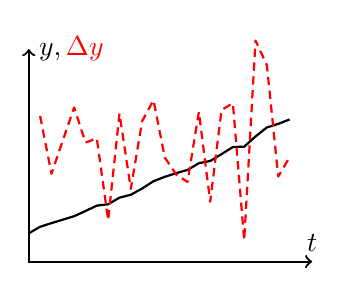
\begin{tikzpicture}[scale=0.18]
	\draw [thick, <->] (0, 15) node [anchor=west] {\( y, {\color{red} \Delta y} \)} -- (0, 0) -- (20, 0) node [anchor=south] {\( t \)}; 
	\draw [thick, black] 
	(0.0, 2.000) -- (0.8, 2.459) -- 
	(1.6, 2.716) -- (3.2, 3.205) -- 
	(4.0, 3.571) -- (4.8, 3.952) -- 
	(5.6, 4.047) -- (6.4, 4.514) -- 
	(7.2, 4.719) -- (8.0, 5.160) -- 
	(8.8, 5.674) -- (9.6, 5.987) -- 
	(10.4, 6.242) -- (11.2, 6.471) -- 
	(12.0, 6.944) -- (12.8, 7.104) -- 
	(13.6, 7.584) -- (14.4, 8.087) -- 
	(15.2, 8.112) -- (16.0, 8.834) -- 
	(16.8, 9.470) -- (17.6, 9.718) -- 
	(18.4, 10.032); 
	\draw [thick, red, densely dashed, line join=round]
	(0.8, 10.28) -- (1.6, 6.20) -- 
	(3.2, 10.88) -- (4.0, 8.40) -- 
	(4.8, 8.70) -- (5.6, 2.92) -- 
	(6.4, 10.45) -- (7.2, 5.13) -- 
	(8.0, 9.92) -- (8.8, 11.39) -- 
	(9.6, 7.34) -- (10.4, 6.15) -- 
	(11.2, 5.62) -- (12.0, 10.57) -- 
	(12.8, 4.23) -- (13.6, 10.70) -- 
	(14.4, 11.18) -- (15.2, 1.51) -- 
	(16.0, 15.60) -- (16.8, 13.86) -- 
	(17.6, 6.01) -- (18.4, 7.36);
\end{tikzpicture}

\end{multicols}

\subsubsection*{De raíz unitaria a cambio porcentual}

Cuando una serie I(1) es estrictamente positiva, a menudo se utilizan logaritmos antes de diferenciar para aproximar cambios porcentuales:

\begin{center}
	\( \Delta \log(y_{t}) = \log(y_{t}) - \log(y_{t - 1}) \approx \dfrac{y_t - y_{t - 1}} {y_{t - 1}} \)
\end{center}

\columnbreak

\subsection*{Ergodicidad}

Un proceso estrictamente estacionario \( \{ y_{t} \} \) es \textbf{ergódico} si los promedios temporales convergen a sus promedios muestrales (esperanzas). Esto suele garantizarse mediante una \textbf{mezcla fuerte} (strong mixing), que implica independencia asintótica de eventos lejanos.

\begin{center}
	\( \frac{1}{T} \sum_{t = 1}^{T} y_{t} \underset{a}{\rightarrow} \E(y_{t}) \)
\end{center}

Sin ello, los momentos muestrales pueden no reflejar los momentos poblacionales. Los estimadores son inconsistentes.

\section*{Cointegración}

Dos series I(1) están \textbf{cointegradas} si una combinación lineal de ellas es I(0). Una regresión entre ellas no es espuria, sino que refleja una relación de \textbf{largo plazo}. Las variables cointegradas comparten una tendencia estocástica común.

Por ejemplo, \( \{ x_{t} \} \) y \( \{ y_{t} \} \) son I(1), pero \( y_{t} - \beta x_{t} = u_{t} \) donde \( \{ u_{t} \} \) es I(0). (\( \beta \) es el parámetro cointegrador).

\subsection*{Contraste de cointegración}

\begin{enumerate}[leftmargin=*]
	\item Estimar \( y_{t} = \alpha + \beta x_{t} + \varepsilon_{t} \) y obtener \( \hat{\varepsilon}_{t} \).
	\item Realizar el ADF sobre \( \hat{\varepsilon}_{t} \) con una distribución especial.
	El resultado del contraste es equivalente a:
	\begin{itemize}[leftmargin=*]
		\item \( H_{0} \): \( \beta = 0 \) (no cointegración)
		\item \( H_{1} \): \( \beta \neq 0 \) (cointegración)
	\end{itemize}
	si el estadístico de contraste \( > \) valor crítico, rechazar \( H_{0} \).
\end{enumerate}

\section*{Heterocedasticidad en series temp.}

Afecta al \textbf{supuesto t4}, lo que lleva a que \textbf{MCO no sea eficiente}.

Usar contrastes como el Breusch-Pagan o White, donde \( H_{0} \): No heterocedasticidad. Para que los contrastes funcionen, no ha de existir \textbf{autocorrelación}.

\subsection*{ARCH}

Un modelo de heteroced. condicional autorreg. (ARCH) se usa para analizar una forma de heteroced. dinámica, donde la varianza del error sigue un proceso \( \text{AR}(p) \).

Dado el modelo: \( y_{t} = \beta_{0} + \beta_{1} z_{t} + u_{t} \) donde, hay AR(1) y heterocedasticidad:

\begin{center}
	\( \E(u_{t}^{2} \mid u_{t - 1}) = \alpha_{0} + \alpha_{1} u_{t - 1}^{2} \)
\end{center}

\subsection*{GARCH}

Un modelo ARCH general (GARCH) es similar a ARCH, pero la varianza del error sigue un proceso \( \text{ARMA}(p, q) \).

\end{multicols}

\end{document}